%===========================================================
% 03_trocr.tex - TrOCR高精度识别
%===========================================================

\section{TrOCR高精度识别}

\begin{frame}{TrOCR简介}
    \textbf{TrOCR:} Transformer-based OCR

    \begin{itemize}
        \item 开发者:Microsoft
        \item 架构:ViT (图像编码器) + GPT-2 (文本解码器)
        \item 优势:端到端训练,准确率最高
    \end{itemize}

    \vspace{0.3cm}

    \textbf{模型:}
    \begin{itemize}
        \item trocr-base-handwritten
        \item trocr-large-handwritten
    \end{itemize}
\end{frame}

%-----------------------------------------------------------
% 新增:Transformer架构基础
%-----------------------------------------------------------

\begin{frame}{Transformer架构概述}
    \textbf{Transformer}是一种完全基于注意力机制的序列转换模型

    \begin{center}
    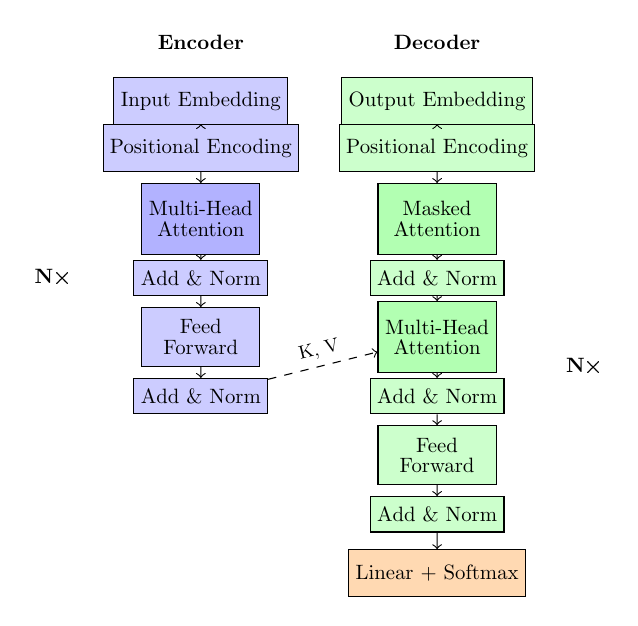
\begin{tikzpicture}[scale=0.75, transform shape]
        % Encoder
        \node[draw, fill=blue!20, minimum width=2cm, minimum height=0.8cm] (enc1) at (0,3) {Input Embedding};
        \node[draw, fill=blue!20, minimum width=2cm, minimum height=0.8cm] (pos1) at (0,2.2) {Positional Encoding};
        \node[draw, fill=blue!30, minimum width=2cm, minimum height=1.2cm] (enc2) at (0,1) {\shortstack{Multi-Head\\Attention}};
        \node[draw, fill=blue!20, minimum width=2cm, minimum height=0.6cm] (norm1) at (0,0) {Add \& Norm};
        \node[draw, fill=blue!20, minimum width=2cm, minimum height=1cm] (ffn) at (0,-1) {\shortstack{Feed\\Forward}};
        \node[draw, fill=blue!20, minimum width=2cm, minimum height=0.6cm] (norm2) at (0,-2) {Add \& Norm};

        % Decoder
        \node[draw, fill=green!20, minimum width=2cm, minimum height=0.8cm] (dec1) at (4,3) {Output Embedding};
        \node[draw, fill=green!20, minimum width=2cm, minimum height=0.8cm] (pos2) at (4,2.2) {Positional Encoding};
        \node[draw, fill=green!30, minimum width=2cm, minimum height=1.2cm] (dec2) at (4,1) {\shortstack{Masked\\Attention}};
        \node[draw, fill=green!20, minimum width=2cm, minimum height=0.6cm] (norm3) at (4,0) {Add \& Norm};
        \node[draw, fill=green!30, minimum width=2cm, minimum height=1.2cm] (dec3) at (4,-1) {\shortstack{Multi-Head\\Attention}};
        \node[draw, fill=green!20, minimum width=2cm, minimum height=0.6cm] (norm4) at (4,-2) {Add \& Norm};
        \node[draw, fill=green!20, minimum width=2cm, minimum height=1cm] (ffn2) at (4,-3) {\shortstack{Feed\\Forward}};
        \node[draw, fill=green!20, minimum width=2cm, minimum height=0.6cm] (norm5) at (4,-4) {Add \& Norm};

        % Output
        \node[draw, fill=orange!30, minimum width=2cm, minimum height=0.8cm] (out) at (4,-5) {Linear + Softmax};

        % Arrows encoder
        \draw[->] (enc1) -- (pos1);
        \draw[->] (pos1) -- (enc2);
        \draw[->] (enc2) -- (norm1);
        \draw[->] (norm1) -- (ffn);
        \draw[->] (ffn) -- (norm2);

        % Arrows decoder
        \draw[->] (dec1) -- (pos2);
        \draw[->] (pos2) -- (dec2);
        \draw[->] (dec2) -- (norm3);
        \draw[->] (norm3) -- (dec3);
        \draw[->] (dec3) -- (norm4);
        \draw[->] (norm4) -- (ffn2);
        \draw[->] (ffn2) -- (norm5);
        \draw[->] (norm5) -- (out);

        % Cross attention
        \draw[->, dashed] (norm2) -- (dec3) node[midway, above, sloped, font=\small] {K, V};

        % Labels
        \node[font=\bfseries] at (0,4) {Encoder};
        \node[font=\bfseries] at (4,4) {Decoder};
        \node[font=\bfseries] at (-2.5,0) {N\texttimes};
        \node[font=\bfseries] at (6.5,-1.5) {N\texttimes};
    \end{tikzpicture}
    \end{center}
\end{frame}

\begin{frame}{自注意力机制原理}
    \textbf{自注意力(Self-Attention)}:计算序列中每个位置与其他所有位置的关联强度

    \vspace{0.3cm}

    \textbf{核心公式:}
    $$\text{Attention}(Q, K, V) = \text{softmax}\left(\frac{QK^T}{\sqrt{d_k}}\right)V$$

    \vspace{0.3cm}

    \begin{columns}
        \begin{column}{0.5\textwidth}
            \textbf{Query (Q):}查询向量\\
            \textbf{Key (K):}键向量\\
            \textbf{Value (V):}值向量
        \end{column}
        \begin{column}{0.5\textwidth}
            \begin{itemize}
                \item $QK^T$:计算相似度
                \item $\sqrt{d_k}$:缩放因子
                \item softmax:归一化为概率
                \item 加权求和得到输出
            \end{itemize}
        \end{column}
    \end{columns}
\end{frame}

\begin{frame}{多头注意力机制}
    \textbf{多头注意力(Multi-Head Attention)}:并行计算多组自注意力,捕获不同子空间的信息

    \vspace{0.3cm}

    $$\text{MultiHead}(Q, K, V) = \text{Concat}(\text{head}_1, ..., \text{head}_h)W^O$$

    $$\text{where } \text{head}_i = \text{Attention}(QW_i^Q, KW_i^K, VW_i^V)$$

    \vspace{0.3cm}

    \begin{center}
    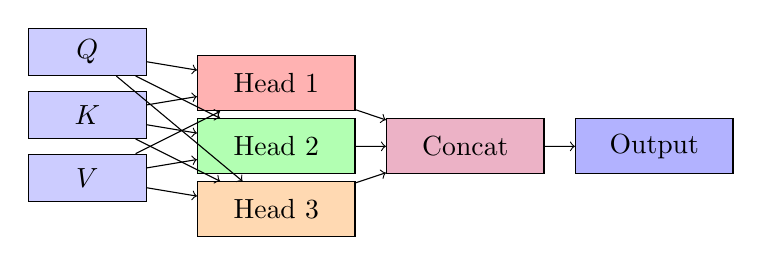
\begin{tikzpicture}[scale=0.8]
        % Input
        \node[draw, fill=blue!20, minimum width=1.5cm, minimum height=0.6cm] (q) at (0,3) {$Q$};
        \node[draw, fill=blue!20, minimum width=1.5cm, minimum height=0.6cm] (k) at (0,2) {$K$};
        \node[draw, fill=blue!20, minimum width=1.5cm, minimum height=0.6cm] (v) at (0,1) {$V$};

        % Heads
        \foreach \i/\y/\c in {1/2.5/red, 2/1.5/green, 3/0.5/orange} {
            \node[draw, fill=\c!30, minimum width=2cm, minimum height=0.7cm] (h\i) at (3,\y) {Head \i};
        }

        % Concat and output
        \node[draw, fill=purple!30, minimum width=2cm, minimum height=0.7cm] (concat) at (6,1.5) {Concat};
        \node[draw, fill=blue!30, minimum width=2cm, minimum height=0.7cm] (out) at (9,1.5) {Output};

        % Arrows
        \foreach \h in {1,2,3} {
            \draw[->] (q) -- (h\h);
            \draw[->] (k) -- (h\h);
            \draw[->] (v) -- (h\h);
            \draw[->] (h\h) -- (concat);
        }
        \draw[->] (concat) -- (out);
    \end{tikzpicture}
    \end{center}
\end{frame}

%-----------------------------------------------------------
% 新增:ViT编码器原理
%-----------------------------------------------------------

\begin{frame}{Vision Transformer (ViT) 架构}
    \textbf{ViT}将Transformer应用于图像分类,TrOCR使用ViT作为图像编码器

    \vspace{0.3cm}

    \textbf{核心思想:}将图像分割成固定大小的块(Patches),将每个块视为一个"词"

    \vspace{0.3cm}

    \begin{center}
    \begin{tikzpicture}[scale=0.7]
        % Original image
        \node at (-3, 2) {原始图像};
        \draw[fill=gray!30] (-4, 0) rectangle (-2, 2);
        \draw[step=0.5] (-4, 0) grid (-2, 2);
        \node at (-3, -0.5) {$224 \times 224$};

        % Arrow
        \draw[->, thick] (-1.5, 1) -- (-0.5, 1) node[midway, above] {分块};

        % Patches
        \node at (2, 2) {图像块序列};
        \foreach \x/\i in {0.5/1, 1.3/2, 2.1/3, 2.9/4, 3.7/5} {
            \draw[fill=blue!20] (\x, 1.2) rectangle (\x+0.6, 1.8);
            \node at (\x+0.3, 1.5) {\tiny $p_\i$};
        }
        \node at (2.5, 0.7) {$\cdots$};

        % Arrow
        \draw[->, thick] (4.5, 1) -- (5.5, 1) node[midway, above] {嵌入};

        % Embeddings
        \node at (7.5, 2) {向量序列};
        \foreach \x/\i in {6.5/1, 7.3/2, 8.1/3, 8.9/4} {
            \draw[fill=green!20] (\x, 1) rectangle (\x+0.6, 1.6);
            \node at (\x+0.3, 1.3) {\tiny $e_\i$};
        }
        \node at (8, 0.5) {$\cdots$};
    \end{tikzpicture}
    \end{center}
\end{frame}

\begin{frame}{ViT编码器结构详解}
    \textbf{ViT编码器的主要组件:}

    \vspace{0.3cm}

    \begin{enumerate}
        \item \textbf{图像分块(Patch Embedding)}
        $$x_p = \text{Flatten}(x_{p}^{(H)} \times x_{p}^{(W)}) \cdot E$$
        其中 $E \in \mathbb{R}^{(P^2 \cdot C) \times D}$ 是可学习的嵌入矩阵

        \vspace{0.2cm}

        \item \textbf{类别Token([CLS] Token)}
        $$z_0 = [x_{\text{class}}; x_p^1E; x_p^2E; \cdots; x_p^NE] + E_{\text{pos}}$$

        \vspace{0.2cm}

        \item \textbf{Transformer编码器层}
        $$z'_{\ell} = \text{MSA}(\text{LN}(z_{\ell-1})) + z_{\ell-1}$$
        $$z_{\ell} = \text{MLP}(\text{LN}(z'_{\ell})) + z'_{\ell}$$
    \end{enumerate}
\end{frame}

\begin{frame}{ViT与CNN编码器对比}
    \begin{columns}
        \begin{column}{0.5\textwidth}
            \textbf{CNN编码器}
            \begin{itemize}
                \item 局部感受野
                \item 平移等变性
                \item 归纳偏置强
                \item 需要大量卷积层提取全局信息
                \item 计算效率高
            \end{itemize}

            \vspace{0.3cm}

            \begin{center}
            \begin{tikzpicture}[scale=0.5]
                \draw[fill=red!20] (0,0) grid (4,4) rectangle (0,0);
                \draw[fill=blue!50] (1,2) rectangle (2,3);
                \node at (0.5, 3.5) {\tiny 局部};
            \end{tikzpicture}
            \end{center}
        \end{column}

        \begin{column}{0.5\textwidth}
            \textbf{ViT编码器}
            \begin{itemize}
                \item 全局感受野
                \item 自注意力机制
                \item 归纳偏置弱
                \item 直接建模全局关系
                \item 数据需求大
            \end{itemize}

            \vspace{0.3cm}

            \begin{center}
            \begin{tikzpicture}[scale=0.5]
                \draw[fill=blue!20] (0,0) grid (4,4) rectangle (0,0);
                \foreach \i in {0,1,2,3} {
                    \foreach \j in {0,1,2,3} {
                        \draw[->, red, thin] (\i+0.5, \j+0.5) -- (2.5, 2.5);
                    }
                }
                \node at (0.5, 3.5) {\tiny 全局};
            \end{tikzpicture}
            \end{center}
        \end{column}
    \end{columns}
\end{frame}

%-----------------------------------------------------------
% 新增:GPT-2解码器原理
%-----------------------------------------------------------

\begin{frame}{GPT-2解码器架构}
    \textbf{GPT-2(Generative Pre-trained Transformer 2)}作为TrOCR的文本解码器

    \vspace{0.3cm}

    \textbf{核心特点:}
    \begin{itemize}
        \item \textbf{仅解码器结构:}使用Masked Self-Attention,只能看到当前位置之前的信息
        \item \textbf{自回归生成:}逐个字符预测,每个新字符依赖于已生成的序列
        \item \textbf{位置编码:}使用可学习的位置嵌入
    \end{itemize}

    \vspace{0.3cm}

    \textbf{解码过程:}
    \begin{align*}
        h_0 &= W_e \cdot x + W_p \\
        h_l &= \text{TransformerBlock}(h_{l-1}), \quad l = 1, \ldots, n \\
        P(y_i | y_{<i}) &= \text{softmax}(W_e^T h_n^{(i)})
    \end{align*}
\end{frame}

\begin{frame}{自回归生成与解码策略}
    \textbf{自回归生成过程:}

    \begin{center}
    \begin{tikzpicture}[scale=0.9, transform shape]
        % Tokens
        \node[draw, fill=green!20, minimum width=1cm, minimum height=0.6cm] (sos) at (0,0) {<sos>};
        \node[draw, fill=blue!20, minimum width=1cm, minimum height=0.6cm] (t1) at (1.5,0) {"H"};
        \node[draw, fill=blue!20, minimum width=1cm, minimum height=0.6cm] (t2) at (3,0) {"e"};
        \node[draw, fill=blue!20, minimum width=1cm, minimum height=0.6cm] (t3) at (4.5,0) {"l"};
        \node[draw, fill=blue!20, minimum width=1cm, minimum height=0.6cm] (t4) at (6,0) {"l"};
        \node[draw, fill=blue!20, minimum width=1cm, minimum height=0.6cm] (t5) at (7.5,0) {"o"};
        \node[draw, fill=red!20, minimum width=1cm, minimum height=0.6cm] (eos) at (9,0) {<eos>};

        % Arrows
        \draw[->] (sos) -- (t1);
        \draw[->] (t1) -- (t2);
        \draw[->] (t2) -- (t3);
        \draw[->] (t3) -- (t4);
        \draw[->] (t4) -- (t5);
        \draw[->] (t5) -- (eos);

        % Model
        \node[draw, fill=gray!30, minimum width=8cm, minimum height=0.8cm] (model) at (4.5,2) {GPT-2 Decoder};

        % Connections to model
        \foreach \x in {0,1.5,3,4.5,6,7.5} {
            \draw[->, gray] (\x,0.5) -- (\x,1.6);
        }

        % Prediction
        \node at (4.5,-1) {每次预测下一个最可能的字符};
    \end{tikzpicture}
    \end{center}

    \vspace{0.3cm}

    \textbf{常用解码策略:}
    \begin{itemize}
        \item \textbf{贪心解码(Greedy):}每次选择概率最高的词
        \item \textbf{束搜索(Beam Search):}保留top-k个候选序列
        \item \textbf{采样解码:}按概率分布随机采样,配合温度参数
    \end{itemize}
\end{frame}

%-----------------------------------------------------------
% 新增:TrOCR训练与微调
%-----------------------------------------------------------

\begin{frame}{TrOCR预训练过程}
    \textbf{TrOCR采用两阶段预训练策略:}

    \vspace{0.3cm}

    \textbf{阶段一:图像编码器预训练(ViT)}
    \begin{itemize}
        \item 数据集:ImageNet-21k
        \item 任务:图像分类
        \item 目标:学习通用的视觉特征表示
    \end{itemize}

    \vspace{0.3cm}

    \textbf{阶段二:端到端文本识别预训练}
    \begin{itemize}
        \item 数据集:
        \begin{itemize}
            \item 合成数据:Synthetically generated handwritten text (数百GB)
            \item 真实数据:IAM, CVL, RIMES等手写数据集
        \end{itemize}
        \item 目标:学习从图像到文本的映射
    \end{itemize}
\end{frame}

\begin{frame}{TrOCR微调方法}
    \textbf{在特定任务上微调TrOCR的常用策略:}

    \vspace{0.3cm}

    \begin{columns}
        \begin{column}{0.55\textwidth}
            \textbf{1. 全模型微调(Full Fine-tuning)}
            \begin{itemize}
                \item 解冻所有参数
                \item 学习率:$5e-6$ 到 $1e-5$
                \item 适合:数据充足的场景
            \end{itemize}

            \vspace{0.3cm}

            \textbf{2. 冻结编码器微调}
            \begin{itemize}
                \item 冻结ViT编码器
                \item 只微调GPT-2解码器
                \item 适合:数据有限的场景
            \end{itemize}
        \end{column}

        \begin{column}{0.45\textwidth}
            \textbf{3. 增量学习}
            \begin{itemize}
                \item 在新数据上继续预训练
                \item 保持原有知识
                \item 逐步适应新领域
            \end{itemize}

            \vspace{0.3cm}

            \textbf{关键超参数:}
            \begin{itemize}
                \item Batch size: 8-32
                \item Epochs: 5-20
                \item Learning rate: $1e-6$ 到 $5e-5$
                \item Warmup steps: 100-500
                \item Weight decay: 0.01
            \end{itemize}
        \end{column}
    \end{columns}
\end{frame}

\begin{frame}{微调数据集准备}
    \textbf{准备用于微调TrOCR的数据集:}

    \vspace{0.3cm}

    \textbf{1. 数据格式}
    \begin{lstlisting}[language=python, basicstyle=\ttfamily\tiny]
# 目录结构
dataset/
  train/
    image_001.jpg
    image_002.jpg
    ...
  val/
    image_101.jpg
    ...
  train_labels.txt  # 格式: 文件名\t文本
  val_labels.txt

# labels.txt 示例
image_001.jpg\t这是一个手写文字示例
image_002.jpg\tHello World
    \end{lstlisting}

    \vspace{0.3cm}

    \textbf{2. 数据增强策略}
    \begin{itemize}
        \item 随机旋转(-5° 到 +5°)
        \item 随机缩放(0.95x 到 1.05x)
        \item 高斯噪声添加
        \item 随机亮度/对比度调整
    \end{itemize}
\end{frame}

%-----------------------------------------------------------
% 原始TrOCR使用代码(保留)
%-----------------------------------------------------------

\begin{frame}[fragile]{TrOCR使用}
    \begin{lstlisting}
# TODO: 使用AI助手补全TrOCR手写识别代码
# 提示词:"使用TrOCR进行手写文字识别的完整流程"
from transformers import TrOCRProcessor, VisionEncoderDecoderModel
from PIL import Image

# TODO: 加载TrOCR处理器和模型
# 提示词:"TrOCRProcessor和VisionEncoderDecoderModel的from_pretrained用法"
processor = TrOCRProcessor.from_pretrained('microsoft/__________')
model = VisionEncoderDecoderModel.from_pretrained('microsoft/__________')

# TODO: 读取图像并进行预处理
# 提示词:"PIL Image.open和TrOCRProcessor的图像预处理"
image = Image.open('__________')
pixel_values = processor(images=image, return_tensors="__________").pixel_values

# TODO: 生成识别结果
# 提示词:"VisionEncoderDecoderModel的generate方法"
generated_ids = model.generate(__________)

# TODO: 解码生成结果
# 提示词:"TrOCRProcessor的batch_decode用法"
text = processor.batch_decode(generated_ids, skip_special_tokens=__________)[0]
    \end{lstlisting}
\end{frame}

%-----------------------------------------------------------
% 新增:扩充代码(GPU/CPU切换、批处理优化等)
%-----------------------------------------------------------

\begin{frame}[fragile]{扩充代码:设备自动切换与优化}
    \begin{lstlisting}[language=python, basicstyle=\ttfamily\tiny]
# TODO: 使用AI助手补全TrOCRRecognizer类的初始化代码
# 提示词:"实现TrOCRRecognizer类的__init__方法,支持自动设备检测和模型加载"
import torch
from transformers import TrOCRProcessor, VisionEncoderDecoderModel
from PIL import Image
import time

class TrOCRRecognizer:
    def __init__(self, model_name='microsoft/trocr-base-handwritten', device=None):
        """
        初始化TrOCR识别器
        :param model_name: 模型名称
        :param device: 指定设备 ('cuda', 'cpu', 或 None自动检测)
        """
        # TODO: 实现设备自动检测
        # 提示词:"PyTorch自动检测GPU/CPU设备的代码"
        if device is None:
            self.device = torch.device('__________' if torch.cuda.__________() else '__________')
        else:
            self.device = torch.device(device)
        print(f"使用设备: {self.device}")

        # TODO: 加载模型和处理器
        # 提示词:"TrOCRProcessor和VisionEncoderDecoderModel的from_pretrained加载"
        print("加载模型中...")
        self.processor = TrOCRProcessor.from_pretrained(__________)
        self.model = VisionEncoderDecoderModel.from_pretrained(__________)
        # TODO: 将模型移动到指定设备并设置为评估模式
        self.model.to(self.device)
        self.model.__________()  # 设置为评估模式

    @torch.no_grad()  # 禁用梯度计算以节省内存
    def recognize(self, image_path):
        """单张图像识别"""
        # TODO: 实现单张图像识别流程
        # 提示词:"使用TrOCR进行单张图像识别的完整步骤"
        image = Image.open(image_path).convert('__________')
        pixel_values = self.processor(images=image, return_tensors="__________").pixel_values.to(self.device)
        generated_ids = self.model.generate(__________)
        text = self.processor.batch_decode(generated_ids, skip_special_tokens=__________)[0]
        return text
    \end{lstlisting}
\end{frame}

\begin{frame}[fragile]{扩充代码:批处理与置信度评估}
    \begin{lstlisting}[language=python, basicstyle=\ttfamily\tiny]
    def recognize_batch(self, image_paths, batch_size=8):
        """
        批量图像识别,优化GPU利用率
        :param image_paths: 图像路径列表
        :param batch_size: 批处理大小
        :return: 识别结果列表 [(path, text, confidence), ...]
        """
        # TODO: 实现批量图像识别
        # 提示词:"使用TrOCR进行批量图像识别的完整流程"
        results = []
        for i in range(0, len(image_paths), batch_size):
            # TODO: 获取当前批次的路径和图像
            batch_paths = image_paths[i:__________]
            batch_images = [Image.open(p).convert('__________') for p in batch_paths]
            # TODO: 批量处理图像
            pixel_values = self.processor(
                images=batch_images,
                return_tensors="__________",
                padding=True
            ).pixel_values.to(self.device)
            # TODO: 生成识别结果并获取分数
            outputs = self.model.generate(
                pixel_values,
                max_length=128,
                num_beams=4,
                output_scores=__________,
                return_dict_in_generate=__________,
                early_stopping=True
            )
            # TODO: 解码文本并计算置信度
            generated_ids = outputs.__________
            texts = self.processor.batch_decode(generated_ids, skip_special_tokens=True)
            for path, text in zip(batch_paths, texts):
                results.append((path, text, 0.0))
        return results

    def recognize_with_confidence(self, image_path):
        """
        带置信度评估的单张图像识别
        :return: (识别文本, 置信度分数, 字符级置信度)
        """
        image = Image.open(image_path).convert('RGB')

        pixel_values = self.processor(
            images=image,
            return_tensors="pt"
        ).pixel_values.to(self.device)

        # 获取生成结果和分数
        outputs = self.model.generate(
            pixel_values,
            max_length=128,
            num_beams=4,
            output_scores=True,
            return_dict_in_generate=True,
            early_stopping=True
        )

        generated_ids = outputs.sequences[0]
        text = self.processor.decode(generated_ids, skip_special_tokens=True)

        # 计算序列级置信度
        sequence_score = outputs.sequences_scores[0] if hasattr(outputs, 'sequences_scores') else 0
        sequence_confidence = torch.exp(sequence_score).item()

        return text, sequence_confidence
    \end{lstlisting}
\end{frame}

\begin{frame}[fragile]{扩充代码:完整错误处理与使用示例}
    \begin{lstlisting}[language=python, basicstyle=\ttfamily\tiny]
# TODO: 使用AI助手补全TrOCRRecognizer类的完整实现
# 提示词:"设计一个支持错误处理和置信度评估的TrOCR识别类"
def safe_recognize(self, image_path):
    """
    带完整错误处理的识别方法
    :return: (success, result, error_message)
    """
    # TODO: 添加文件存在性检查
    # 提示词:"Python检查文件是否存在的方法"
    import os
    if not os.__________(image_path):
        return False, None, f"文件不存在: {image_path}"

    # TODO: 添加文件格式验证
    # 提示词:"检查文件扩展名的Python代码"
    valid_extensions = ('.jpg', '.jpeg', '.png', '.bmp', '.tiff')
    if not image_path.lower().__________(valid_extensions):
        return False, None, f"不支持的文件格式"

    # TODO: 实现图像打开和尺寸检查
    # 提示词:"PIL Image打开图像并获取尺寸"
    try:
        image = Image.open(image_path)
        width, height = image.size
    except Exception as e:
        return False, None, f"无法打开图像: {str(e)}"

    # TODO: 调用识别方法并返回结构化结果
    # 提示词:"调用recognize_with_confidence并组装结果字典"
    text, confidence = self.__________(image_path)
    result = {
        'text': __________,
        'confidence': __________,
        'image_size': (width, height)
    }
    return True, result, None

# TODO: 使用AI助手补全主程序使用示例
# 提示词:"TrOCRRecognizer类的初始化与调用示例"
if __name__ == "__________":
    # TODO: 初始化识别器
    recognizer = TrOCRRecognizer(
        model_name='microsoft/__________'
    )
    # TODO: 调用safe_recognize并处理结果
    success, result, error = recognizer.__________("handwriting.jpg")
    if success:
        print(f"识别结果: {result['__________']}")
        print(f"置信度: {result['__________']:.4f}")
    else:
        print(f"识别失败: {error}")
    \end{lstlisting}
\end{frame}

\begin{frame}[fragile]{TrOCR批量识别}
    \begin{lstlisting}
# TODO: 使用AI助手补全TrOCR批量识别代码
# 提示词:"使用TrOCR进行批量手写文字识别的完整流程"
from transformers import TrOCRProcessor, VisionEncoderDecoderModel
from PIL import Image
import torch

# TODO: 加载TrOCR处理器和模型
# 提示词:"TrOCRProcessor和VisionEncoderDecoderModel的from_pretrained用法"
processor = TrOCRProcessor.from_pretrained('microsoft/__________')
model = VisionEncoderDecoderModel.from_pretrained('microsoft/__________')

# TODO: 定义待识别的图像路径列表
# 提示词:"Python列表定义多个图像文件路径"
image_paths = ['__________', '__________', '__________']
results = []

# TODO: 实现批量识别的循环
# 提示词:"遍历图像列表并使用TrOCR进行识别的代码"
for path in image_paths:
    # TODO: 打开图像并转换颜色模式
    image = Image.open(path).__________
    # TODO: 使用processor预处理图像
    pixel_values = processor(images=image, return_tensors="__________").pixel_values
    # TODO: 使用模型生成识别结果
    generated_ids = model.__________(pixel_values)
    # TODO: 解码生成结果为文本
    text = processor.batch_decode(generated_ids, skip_special_tokens=__________)[0]
    # TODO: 保存结果并打印
    results.append((path, text))
    print(f"{path}: {text}")
    \end{lstlisting}
\end{frame}

\begin{frame}{PaddleOCR vs TrOCR对比}
    \begin{table}
        \centering
        \begin{tabular}{lcc}
            \toprule
            \textbf{特性} & \textbf{PaddleOCR} & \textbf{TrOCR} \\
            \midrule
            准确率 & 85-90\% & \textbf{95\%+} \\
            速度 & \textbf{快} & 慢 \\
            中文支持 & \textbf{原生支持} & 一般 \\
            部署难度 & \textbf{简单} & 复杂 \\
            GPU需求 & 低 & \textbf{高} \\
            \bottomrule
        \end{tabular}
    \end{table}

    \textbf{选择建议:}
    \begin{itemize}
        \item 追求准确率 $\to$ TrOCR
        \item 追求速度/易用 $\to$ PaddleOCR
    \end{itemize}
\end{frame}
